%% abtex2-modelo-trabalho-academico.tex, v-1.9.5 laurocesar
%% Copyright 2012-2015 by abnTeX2 group at http://www.abntex.net.br/ 
%%
%% This work may be distributed and/or modified under the
%% conditions of the LaTeX Project Public License, either version 1.3
%% of this license or (at your option) any later version.
%% The latest version of this license is in
%%   http://www.latex-project.org/lppl.txt
%% and version 1.3 or later is part of all distributions of LaTeX
%% version 2005/12/01 or later.
%%
%% This work has the LPPL maintenance status `maintained'.
%% 
%% The Current Maintainer of this work is the abnTeX2 team, led
%% by Lauro César Araujo. Further information are available on 
%% http://www.abntex.net.br/
%%
%% This work consists of the files abntex2-modelo-trabalho-academico.tex,
%% abntex2-modelo-include-comandos and abntex2-modelo-references.bib
%%

% ------------------------------------------------------------------------
% ------------------------------------------------------------------------
% abnTeX2: Modelo de Trabalho Academico (tese de doutorado, dissertacao de
% mestrado e trabalhos monograficos em geral) em conformidade com 
% ABNT NBR 14724:2011: Informacao e documentacao - Trabalhos academicos -
% Apresentacao
% ------------------------------------------------------------------------
% ------------------------------------------------------------------------
\PassOptionsToPackage{hyperfootnotes=false}{hyperref}

\documentclass[
	% -- opções da classe memoir --
	12pt,				% tamanho da fonte
	openright,			% capítulos começam em pág ímpar (insere página vazia caso preciso)
	twoside,			% para impressão em verso e anverso. Oposto a oneside
	a4paper,			% tamanho do papel. 
	% -- opções da classe abntex2 --
	%chapter=TITLE,		% títulos de capítulos convertidos em letras maiúsculas
	%section=TITLE,		% títulos de seções convertidos em letras maiúsculas
	%subsection=TITLE,	% títulos de subseções convertidos em letras maiúsculas
	%subsubsection=TITLE,% títulos de subsubseções convertidos em letras maiúsculas
	% -- opções do pacote babel --
	english,			% idioma adicional para hifenização
	french,				% idioma adicional para hifenização
	spanish,			% idioma adicional para hifenização
	brazil				% o último idioma é o principal do documento
	]{abntex2}

% ---
% Pacotes básicos 
% ---
\usepackage{lmodern}			% Usa a e Latin Modern			
\usepackage[T1]{fontenc}		% Selecao de codigos de fonte.
\usepackage[utf8]{inputenc}		% Codificacao do documento (conversão automática dos acentos)
\usepackage{lastpage}			% Usado pela Ficha catalográfica
\usepackage{indentfirst}		% Indenta o primeiro parágrafo de cada seção.
\usepackage{color}				% Controle das cores
\usepackage{graphicx}			% Inclusão de gráficos
\usepackage{microtype} 			% para melhorias de justificação
% ---

\usepackage{afterpage}			% Pacote utilizado para colocar referencia de figura na mesma páginad a figura

\usepackage{float}

\usepackage{pdfpages}


% ---
% Pacotes adicionais, usados apenas no âmbito do Modelo Canônico do abnteX2
% ---
\usepackage{lipsum}				% para geração de dummy text
% ---

% ---
% Pacotes de citações
% ---
\usepackage[brazilian,hyperpageref]{backref}	 % Paginas com as citações na bibl
\usepackage[alf]{abntex2cite}	% Citações padrão ABNT

\usepackage[hang, flushmargin]{footmisc} % pacote de formatação para footnotes
\usepackage[all]{hypcap}

\let\svthefootnote\thefootnote
\setlength\footnotemargin{10pt}

% --- 
% CONFIGURAÇÕES DE PACOTES
% --- 

% ---
% Configurações do pacote backref
% Usado sem a opção hyperpageref de backref
\renewcommand{\backrefpagesname}{Citado na(s) página(s):~}
% Texto padrão antes do número das páginas
\renewcommand{\backref}{}
% Define os textos da citação
\renewcommand*{\backrefalt}[4]{
	\ifcase #1 %
		Nenhuma citação no texto.%
	\or
		Citado na página #2.%
	\else
		Citado #1 vezes nas páginas #2.%
	\fi}%
% ---


% Editar estilo da capa
\renewcommand{\imprimircapa}{%
	\begin{capa}%
		\center
	%	\ABNTEXchapterfont\Large UNIVERSIDADE QUE TORNA OS DOCUMENTOS AINDA
	%	MAIS ESTRANHOS
		\vspace*{1cm}
		{\ABNTEXchapterfont\large\imprimirautor}
		\vfill
		\begin{center}
			\ABNTEXchapterfont\bfseries\LARGE\imprimirtitulo
		\end{center}
		\vfill
		\begin{flushright}
			\ABNTEXchapterfont Aluno: Dennis Teles dos Santos \\
			\ABNTEXchapterfont RA: 09.03046-8 \\
			\ABNTEXchapterfont Curso: Engenharia Eletrônica \\
			\ABNTEXchapterfont Série: 6º ano
		\end{flushright}
		\vfill
		\large\imprimirlocal \\
		\large\imprimirdata
		\vspace*{1cm}
	\end{capa}
}
% ---

% ---

% if your original example included a URL that has that specific structure, then it will solve your problem. 
\makeatletter
\g@addto@macro{\UrlBreaks}{\UrlOrds}
\makeatother		
% ---

% ---
% Informações de dados para CAPA e FOLHA DE ROSTO
% ---

\titulo{Relatório do Estágio Supervisionado}
\autor{Dennis Teles dos Santos}
\local{São Caetano Do Sul}
\data{2015}
\orientador{Vanderlei Cunha Parro}
\coorientador{Rafael Corsi Ferrão}
\instituicao{%
  Instituto Mauá de Tecnologia -- IMT
  \par
  Engenharia Eletrônica
  \par
  Programa de Iniciação Científica}
\tipotrabalho{Relatório de Estágio Supervisionado}
% O preambulo deve conter o tipo do trabalho, o objetivo, 
% o nome da instituição e a área de concentração 
\preambulo{Relatório de estágio apresentado à Escola de Engenharia Mauá do Centro Universitário do Instituto Mauá de Tecnologia como parte da exigência da disciplina Estágio Supervisionado Obrigatório. sob a orientação do Prof. Vanderlei Cunha Parro.}
% ---


% ---
% Configurações de aparência do PDF final

% alterando o aspecto da cor azul
\definecolor{blue}{RGB}{41,5,195}

% informações do PDF
\makeatletter
\hypersetup{
     	%pagebackref=true,
		pdftitle={\@title}, 
		pdfauthor={\@author},
    	pdfsubject={\imprimirpreambulo},
	    pdfcreator={LaTeX with abnTeX2},
		pdfkeywords={abnt}{latex}{abntex}{abntex2}{trabalho acadêmico}, 
		colorlinks=true,       		% false: boxed links; true: colored links
    	linkcolor=blue,          	% color of internal links
    	citecolor=blue,        		% color of links to bibliography
    	filecolor=magenta,      		% color of file links
		urlcolor=blue,
		bookmarksdepth=4
}
\makeatother
% --- 


% --- 
% Espaçamentos entre linhas e parágrafos 
% --- 

% O tamanho do parágrafo é dado por:
\setlength{\parindent}{1.3cm}

% Controle do espaçamento entre um parágrafo e outro:
\setlength{\parskip}{0.2cm}  % tente também \onelineskip

% ---
% compila o indice
% ---
\makeindex
% ---

% ----
% Início do documento
% ----
\begin{document}

% Seleciona o idioma do documento (conforme pacotes do babel)
%\selectlanguage{english}
\selectlanguage{brazil}

% Retira espaço extra obsoleto entre as frases.
\frenchspacing 

% ----------------------------------------------------------
% ELEMENTOS PRÉ-TEXTUAIS
% ----------------------------------------------------------
% \pretextual

% ---
% Capa
% ---
\imprimircapa
% ---

% ---
% Folha de rosto
% (o * indica que haverá a ficha bibliográfica)
% ---
\imprimirfolhaderosto*
% ---

% ---
% Inserir a ficha bibliografica
% ---

% Isto é um exemplo de Ficha Catalográfica, ou ``Dados internacionais de
% catalogação-na-publicação''. Você pode utilizar este modelo como referência. 
% Porém, provavelmente a biblioteca da sua universidade lhe fornecerá um PDF
% com a ficha catalográfica definitiva após a defesa do trabalho. Quando estiver
% com o documento, salve-o como PDF no diretório do seu projeto e substitua todo
% o conteúdo de implementação deste arquivo pelo comando abaixo:
%
% \begin{fichacatalografica}
%     \includepdf{fig_ficha_catalografica.pdf}
% \end{fichacatalografica}

\begin{fichacatalografica}
	\sffamily
	\vspace*{\fill}					% Posição vertical
	\begin{center}					% Minipage Centralizado
	\fbox{\begin{minipage}[c][8cm]{13.5cm}		% Largura
	\small
	%\imprimirautor
	Santos, Dennis Teles dos
	%Sobrenome, Nome do autor
	
	\hspace{0.5cm} \imprimirtitulo  / \imprimirautor. --
	\imprimirlocal, \imprimirdata-
	
	\hspace{0.5cm} \pageref{LastPage} p. : il. (algumas color.) ; 30 cm.\\
	
	\hspace{0.5cm} \imprimirorientadorRotulo~\imprimirorientador\\
	
	\hspace{0.5cm}
	\parbox[t]{\textwidth}{\imprimirtipotrabalho~--~\imprimirinstituicao,
	\imprimirdata.}\\
	
	\hspace{0.5cm}
		1. Aplicação SpaceWire. % Palavra-chave1.
		2. Comunicação aeroespacial. % Palavra-chave2.
		2. Conversores. % Palavra-chave3.
		I. Vanderlei Cunha Parro, % Orientador.
		II. Instituto Mauá de Tecnologia % Universidade xxx.
		III. Faculdade de Engenharia Eletrônica. % Faculdade de xxx.
		IV. Aplicação SpaceWire. % Título 			
	\end{minipage}}
	\end{center}
\end{fichacatalografica}
% ---

\iffalse
% ---
% Inserir errata
% ---
\begin{errata}
Elemento opcional da \citeonline[4.2.1.2]{NBR14724:2011}. Exemplo:

\vspace{\onelineskip}

FERRIGNO, C. R. A. \textbf{Tratamento de neoplasias ósseas apendiculares com
reimplantação de enxerto ósseo autólogo autoclavado associado ao plasma
rico em plaquetas}: estudo crítico na cirurgia de preservação de membro em
cães. 2011. 128 f. Tese (Livre-Docência) - Faculdade de Medicina Veterinária e
Zootecnia, Universidade de São Paulo, São Paulo, 2011.

\begin{table}[htb]
\center
\footnotesize
\begin{tabular}{|p{1.4cm}|p{1cm}|p{3cm}|p{3cm}|}
  \hline
   \textbf{Folha} & \textbf{Linha}  & \textbf{Onde se lê}  & \textbf{Leia-se}  \\
    \hline
    1 & 10 & auto-conclavo & autoconclavo\\
   \hline
\end{tabular}
\end{table}

\end{errata}
% ---
\fi

% ---
% Inserir folha de aprovação
% ---

% Isto é um exemplo de Folha de aprovação, elemento obrigatório da NBR
% 14724/2011 (seção 4.2.1.3). Você pode utilizar este modelo até a aprovação
% do trabalho. Após isso, substitua todo o conteúdo deste arquivo por uma
% imagem da página assinada pela banca com o comando abaixo:
%
% \includepdf{folhadeaprovacao_final.pdf}
%
\begin{folhadeaprovacao}

  \begin{center}
    {\ABNTEXchapterfont\large\imprimirautor}

    \vspace*{\fill}\vspace*{\fill}
    \begin{center}
      \ABNTEXchapterfont\bfseries\Large\imprimirtitulo
    \end{center}
    \vspace*{\fill}
    
    \hspace{.45\textwidth}
    \begin{minipage}{.5\textwidth}
        \imprimirpreambulo
    \end{minipage}%
    \vspace*{\fill}
   \end{center}
        
   Relatório aprovado. \imprimirlocal, \underline{\hspace{0.7cm}} de \underline{\hspace{3.4cm}} de 2015:

   \assinatura{\textbf{\imprimirorientador} \\ Orientador} 
   \assinatura{\textbf{Rodrigo Alvite Romano} \\ Examinador}
   %\assinatura{\textbf{Professor} \\ Convidado 2}
   %\assinatura{\textbf{Professor} \\ Convidado 3}
   %\assinatura{\textbf{Professor} \\ Convidado 4}
      
   \begin{center}
    \vspace*{0.5cm}
    {\large\imprimirlocal}
    \par
    {\large\imprimirdata}
    \vspace*{1cm}
  \end{center}
  
\end{folhadeaprovacao}
% ---

\iffalse
% ---
% Dedicatória
% ---
\begin{dedicatoria}
   \vspace*{\fill}
   \centering
   \noindent
   \textit{ Este trabalho é dedicado às crianças adultas que,\\
   quando pequenas, sonharam em se tornar cientistas.} \vspace*{\fill}
\end{dedicatoria}
% ---
\fi

\iffalse
% ---
% Agradecimentos
% ---
\begin{agradecimentos}
Os agradecimentos principais são direcionados à Gerald Weber, Miguel Frasson,
Leslie H. Watter, Bruno Parente Lima, Flávio de Vasconcellos Corrêa, Otavio Real
Salvador, Renato Machnievscz\footnote{Os nomes dos integrantes do primeiro
projeto abn\TeX\ foram extraídos de
\url{http://codigolivre.org.br/projects/abntex/}} e todos aqueles que
contribuíram para que a produção de trabalhos acadêmicos conforme
as normas ABNT com \LaTeX\ fosse possível.

Agradecimentos especiais são direcionados ao Centro de Pesquisa em Arquitetura
da Informação\footnote{\url{http://www.cpai.unb.br/}} da Universidade de
Brasília (CPAI), ao grupo de usuários
\emph{latex-br}\footnote{\url{http://groups.google.com/group/latex-br}} e aos
novos voluntários do grupo
\emph{\abnTeX}\footnote{\url{http://groups.google.com/group/abntex2} e
\url{http://www.abntex.net.br/}}~que contribuíram e que ainda
contribuirão para a evolução do \abnTeX.

\end{agradecimentos}
% ---
\fi

% ---
% Epígrafe
% ---
\begin{epigrafe}
    \vspace*{\fill}
	\begin{flushright}
		\textit{``Não vos amoldeis às estruturas deste mundo, \\
		mas transformai-vos pela renovação da mente, \\
		a fim de distinguir qual é a vontade de Deus: \\
		o que é bom, o que Lhe é agradável, o que é perfeito.\\
		(Bíblia Sagrada, Romanos 12, 2)}
	\end{flushright}
\end{epigrafe}
% ---

\iffalse

% ---
% RESUMOS
% ---

% resumo em português
\setlength{\absparsep}{18pt} % ajusta o espaçamento dos parágrafos do resumo

\begin{resumo} 
	O projeto visa criar um hardware utilizando como comunicação o protocolo SpaceWire, amplamente utilizado em projetos aeroespaciais, que seja capaz de ler e escrever em conversores analógico-digital e digital-analógico.
	
	O protocolo SpaceWire é uma rede de comunicação criada e coordenada pela agência espacial europeia em colaboração com agências espaciais internacionais. Este protocolo traz muitas vantagens, além de ser facilmente implementado em circuitos integrados de aplicação específica (CIAEs) e transmitir dados com maior segurança e velocidade, ajuda a reduzir custos de integração de sistemas.
	
	A arquitetura do sistema é composta por: um controlador geral, um banco de registradores e módulos de periféricos. O controlador é responsável pelo gerenciamento do sistema e é acessado diretamente pelo codec SpaceWire e pela comunicação serial. O banco de registradores permite o armazenamento de dados e informações de comando para os módulos. Os módulos de periféricos acessam o banco de registradores e controlam os dispositivos externos (leds, entradas e saídas digitais e conversores). O acesso aos conversores é feito através do protocolo de comunicação serial SPI.
	
	Este projeto foi implementado em uma placa de desenvolvimento que contém uma FPGA Xilinx Virtex 5 utilizando programação VHDL. Também foi construído um hardware contendo: entradas e saídas digitais, leds e conversores analógico digital e digital-analógico de dois canais, os quais podem ser conectados a equipamentos como sensor de temperatura e motores de acionamento.
	
	O sistema desenvolvido pode se comunicar a uma rede SpaceWire e todos os dispositivos do hardware possuem acessos através desta comunicação mostrando assim um dos principais benefícios deste protocolo que é promover compatibilidade entre equipamentos e subsistemas.


 \textbf{Palavras-chave}: Aplicação SpaceWire. Comunicação aeroespacial. Conversores.
\end{resumo}

% resumo em inglês
\begin{resumo}[Abstract]
 \begin{otherlanguage*}{english}
    The project aims to create a payload hardware for cubesats using as communication the SpaceWire protocol, widely used in aerospace projects, able to read and write on analog-to-digital and digital-to-analog converters.
    
    SpaceWire protocol is a space communication network created and coordinated by European Space Agency (ESA) in collaboration with international space agencies including NASA, JAXA and RKA. This protocol has many advantages besides being easily implemented in application-specific integrated circuit (ASIC) and transmit data with greater security and speed, it helps to reduce system integration costs.
    
    The system architecture consists of: a general controller, a registers bank and peripheral modules. The controller is responsible for system management and it is accessed directly by SpaceWire codec and serial communication. The registers bank allows the storage of data and control information for the modules. Peripheral modules access the registers bank and control external devices (LEDs, digital inputs and outputs and converters). The access to converters is via SPI serial communication protocol.
    
    This project was implemented in a development board which contains a Xilinx Virtex 5 FPGA using VHDL code. A hardware containing digital inputs and outputs, LEDs and analog-to-digital and digital-to-analog converters of two channels also was builtchannels also was built, which can be connected to devices such as temperature sensors and drive motors..
    
    The developed system can communicate to a SpaceWire network and all hardware devices have access through this communication, thus showing a key benefit of this protocol that is to promote compatibility between devices and subsystems.

   \vspace{\onelineskip}
 
   \noindent 
   \textbf{Keywords}: SpaceWire application. Aerospace communication. Converters.
 \end{otherlanguage*}
\end{resumo}

%	% resumo em francês 
%	\begin{resumo}[Résumé]
%	 \begin{otherlanguage*}{french}
%	    Il s'agit d'un résumé en français.
%	 
%	   \textbf{Mots-clés}: latex. abntex. publication de textes.
%	 \end{otherlanguage*}
%	\end{resumo}
%	
%	% resumo em espanhol
%	\begin{resumo}[Resumen]
%	 \begin{otherlanguage*}{spanish}
%	   Este es el resumen en español.
%	  
%	   \textbf{Palabras clave}: latex. abntex. publicación de textos.
%	 \end{otherlanguage*}
%	\end{resumo}
%	% ---

\fi

\iffalse
% ---
% inserir lista de ilustrações
% ---
\pdfbookmark[0]{\listfigurename}{lof}
\listoffigures*
\cleardoublepage
% ---
\fi

\iffalse
% ---
% inserir lista de tabelas
% ---
\pdfbookmark[0]{\listtablename}{lot}
\listoftables*
\cleardoublepage
% ---
\fi

\iffalse
% ---
% inserir lista de abreviaturas e siglas
% ---
\begin{siglas}
  \item[ABNT] Associação Brasileira de Normas Técnicas
  \item[abnTeX] ABsurdas Normas para TeX
\end{siglas}
% ---
\fi

\iffalse
% ---
% inserir lista de símbolos
% ---
\begin{simbolos}
  \item[$ \Gamma $] Letra grega Gama
  \item[$ \Lambda $] Lambda
  \item[$ \zeta $] Letra grega minúscula zeta
  \item[$ \in $] Pertence
\end{simbolos}
% ---
\fi


% ---
% inserir o sumario
% ---
\pdfbookmark[0]{\contentsname}{toc}
\tableofcontents*
\cleardoublepage
% ---



% ----------------------------------------------------------
% ELEMENTOS TEXTUAIS
% ----------------------------------------------------------
\textual

% ----------------------------------------------------------
% Introdução (exemplo de capítulo sem numeração, mas presente no Sumário)
% ----------------------------------------------------------
\chapter*[Introdução]{Introdução}
\addcontentsline{toc}{chapter}{Introdução}
% ----------------------------------------------------------

	Este relatório tem como objetivo descrever as atividades desenvolvidas por Dennis Teles dos Santos, aluno do Curso de Engenharia Eletrônica da Escola de Engenharia Mauá, como parte da exigência da disciplina Estágio Supervisionado Obrigatório pertencente ao sexto ano do período noturno.
	
	O estágio foi desenvolvido no Núcleo de Sistemas Eletrônicos Embarcados (NSEE) do Instituto Mauá de Tecnologia pelo programa de Iniciação Científica (IC) ligado ao projeto de pesquisa financiado pelo CNPq sob a coordenação do CITAR (Circuitos Integrados Tolerantes à Radiação). O projeto proposto no âmbito da meta 2 - Circuito Integrado SpaceWire visa desenvolver uma aplicação aeroespacial de exemplo (bancada) utilizando o protocolo de comunicação SpaceWire.
	
	O projeto permitiu a realização de atividades relacionadas a área da Engenharia Eletrônica, bem como o uso e aperfeiçoamento do conhecimento adquirido durante o Curso de Engenharia Eletrônica oferecido pela Escola de Engenharia Mauá.
	
	Este relatório contém uma breve descrição sobre o NSEE e o projeto CITAR. Também possui uma descrição detalhada das atividades realizadas pelo aluno durante o período da Iniciação Científica. Por fim, o relatório é encerrado com uma conclusão relativa ao estágio.
	

% ----------------------------------------------------------
% PARTE
% ----------------------------------------------------------
\part{Apresentação da Empresa}
% ----------------------------------------------------------

% ---
% Capitulo da Apresentação da Empresa - Sobre o NSEE
% ---
\chapter{Local da realização das atividades}
As atividades realizadas durante o período do estágio foram feitas no Núcleo de Sistemas Eletrônicos Embarcados (NSEE), laboratório localizado no Instituto Mauá de Tecnologia (IMT). Este capítulo terá uma breve descrição sobre o NSEE e o IMT.
% ---

\section{O Instituto Mauá de Tecnologia (IMT)}
Fundado em 11 de dezembro de 1961, o Instituto Mauá de Tecnologia (IMT) é uma entidade privada, sem fins lucrativos, e dedicada ao ensino e à pesquisa científica e tecnológica, com a finalidade de formar recursos humanos altamente qualificados para a contribuição do desenvolvimento do País.(\uppercase{Instituto...}, S/Data) \let\thefootnote\relax\footnotetext{\uppercase{Instituto} Mauá de Tecnologia. Disponível em:  \url{http://www.institutodeengenharia.org.br/site/universidades/detalhes/id\_sessao/66/id\_universidade/4/Instituto-Mauá-de-Tecnologia}. Acesso em: 8 out. 2015.}

O IMT, com campi em São Paulo e São Caetano do Sul (Figura \ref{IMT}), mantém duas unidades: Centro Universitário e Centro de Pesquisas. O Centro Universitário oferece cursos de graduação em Administração, Design e Engenharia. Na pós-graduação, são oferecidos cursos de aperfeiçoamento, especialização e MBA nas áreas de Administração, Gestão e Engenharia e é desenvolvido programa de Mestrado em processos químicos e bioquímicos. O Centro de Pesquisas, há mais de 45 anos, desenvolve tecnologia para atendimento das necessidades da indústria.(\uppercase{Alunos...}, 2015) \let\thefootnote\relax\footnotetext{\uppercase{Alunos} do Instituto Mauá de Tecnologia iniciam construção de satélite em miniatura para pesquisas espaciais. Disponível em: \url{http://maua.br/imprensa/press-releases/528-alunos-do-imt-iniciam-construcao-de-satelite-em-miniatura-para-pesquisas-espaciais}. Acesso em: 7 out. 2015.}

\let\thefootnote\svthefootnote

\begin{figure}[!htb]
	\centering
	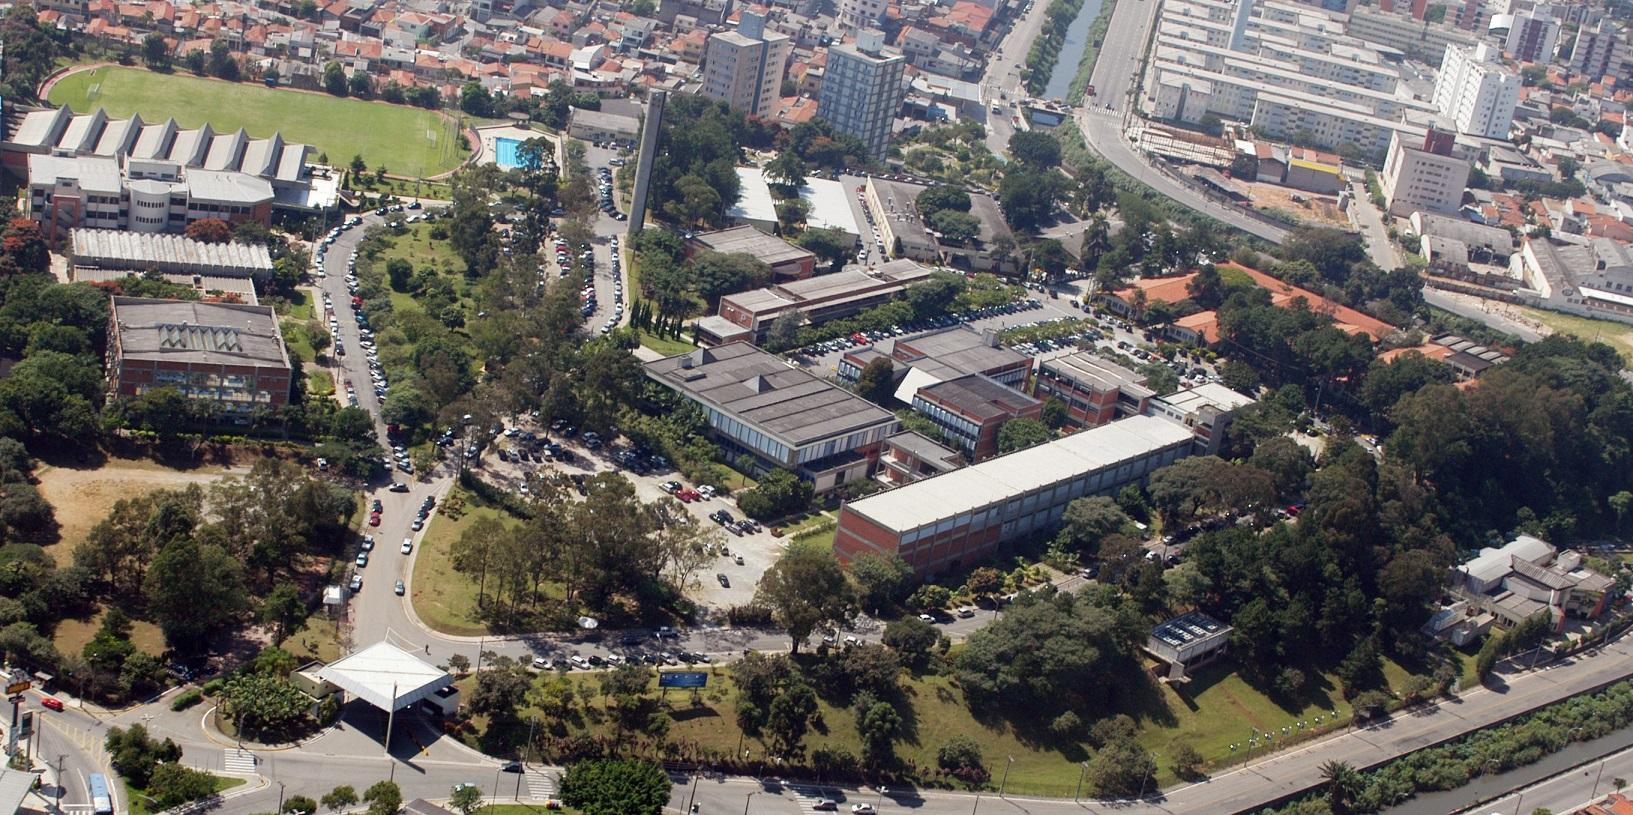
\includegraphics[scale = 1]{Imagens/Campus_IMT_foto_aerea.jpg}
	\caption{Vista aérea do \textit{Campus} do IMT de São Caetano do Sul.}
	\label{IMT}
\end{figure}

% ---

% ---
\section{O Núcleo de Sistemas Eletrônicos Embarcados (NSEE)}
Para saber um pouco mais sobre o novo laboratório Núcleo de Sistemas Eletrônicos Embarcados (NSEE), antes de tudo é preciso entender que sistemas embarcados são uma classe de sistemas digitais voltados e desenvolvidos para aplicações específicas, apresentando, frequentemente, restrições de processamento em tempo real. Apesar da complexidade do tema, esse tipo de tecnologia já faz parte de objetos do nosso cotidiano, como GPS e telefones celulares e vem sendo cada dia mais utilizada nas áreas automotiva, espacial, industrial e de entretenimento.

Criado no início do ano de 2010, o Núcleo coordenado pelo professor Vanderlei Cunha Parro, além de ter como objetivo o estudo e o desenvolvimento desse tipo de sistema, também possui outros temas de interesse, como aplicações em processamento de sinais, controle digital e experimentos aeroespaciais.(\uppercase{Campus...}, 2010) \let\thefootnote\relax\footnotetext{\uppercase{Campus} de São Caetano do Sul tem novo laboratório de Sistemas Eletrônicos Embarcados. Disponível em:  \url{http://maua.br/imprensa/infomaua/29/texto/147}. Acesso em: 7 out. 2015.}

O laboratório possui vários computadores e um amplo espaço para realizações de diversos projetos. Possui também componentes e equipamentos eletrônicos que auxiliam nas diversas tarefas, como fontes de alimentação, multímetro e osciloscópio. Há também o almoxarifado de componentes e equipamentos eletrônicos no piso superior que oferece um suporte a mais ao NSEE e, consequentemente, aos projetos realizados no laboratório. 

O ambiente do NSEE também favorece o estudo e aprendizado. Os alunos e pesquisadores procuram sempre ajudar um ao outro em suas dificuldades fazendo com que todos possam crescer juntos.

% ---

% ---
% Capitulo da Apresentação da Empresa - O CITAR
% ---
\chapter{O projeto CITAR (Circuitos Integrados Tolerantes à Radiação)}
O projeto desenvolvido durante o estágio está no plano da Meta 2 do projeto CITAR. Uma breve descrição sobre o CITAR será apresentada a seguir.

% ---
\section{Sobre o CITAR}
O Centro de Tecnologia da Informação Renato Archer - CTI, inaugurou o Projeto CITAR – Circuitos Integrados Tolerantes à Radiação, no dia 15 de julho de 2013 nas instalações do BBP - Brazilian Business Park, um espaço que abriga o Centro de Inovação da cidade de Atibaia - SP. A cerimônia (Figura \ref{Cerimonia}) contou com a presença do Ministro da Ciência, Tecnologia e Inovação Marco Antonio Raupp, além de outras autoridades.

O Projeto CITAR, conta com financiamento da Agência Brasileira de Inovação - FINEP e é executado em um esforço de cooperação entre o CTI Renato Archer e outras instituições de pesquisa e ensino: o Instituto Nacional de Pesquisas Espaciais (INPE), a Agência Espacial Brasileira (AEB), o Instituto de Física da USP (IFUSP) e o Instituto de Estudos Avançados (IEAv).
Trata-se da primeira ação multinstitucional brasileira para o desenvolvimento de circuitos integrados tolerantes à radiação, destinados a aplicações em satélites científicos, que colocará Atibaia no mapa da produção e desenvolvimento de tecnologia aeroespacial brasileira.

Com um orçamento de R\$ 20 milhões provenientes da FINEP, o projeto CITAR term a duração total de 24 meses e conta com a participação de uma equipe multiprofissional formada por mais de 40 pessoas. Os recursos são utilizados na contratação da equipe de desenvolvimento, capacitação e treinamento de profissionais, aquisição de equipamentos para infraestrutura de projetos e testes e na fabricação e qualificação de componentes. Para o diretor do CTI Renato Archer, Victor Pellegrini Mammana, o projeto é um grande passo para as instituições partícipes e para toda a produção tecnológica brasileira.

Toda essa iniciativa conta com pleno apoio do Governo Federal, na figura do Ministério da Ciência, Tecnologia e Inovação (MCTI), do Conselho Nacional de Desenvolvimento Científico e Tecnológico (CNPq) e do Programa CI Brasil.

O maior objetivo do Projeto CITAR é consolidar, no Brasil, a competência para a realização do ciclo completo de desenvolvimento compreendo as etapas de especificação, projeto, simulação, layout, envio para fabricação, encapsulamento, teste e qualificação de Circuitos Integrados tolerantes a radiações, para aplicações aeroespaciais e afins. As atividades serão focadas no desenvolvimento de CI's demandados pelo programa espacial brasileiro, indicados pelo INPE. (\uppercase{Cenpra}, 2013)\let\thefootnote\relax\footnotetext{Este texto foi retirado da URL \url{http://www.cenpra.gov.br/ultimas-noticias/264-cti-renato-archer-inaugura-projeto-de-tecnologia-espacial-na-cidade-de-atibaia-sp}. Acesso em: 7 out. 2015.}
% ---



\vfill
\begin{figure}[!htb]
	\centering
	\caption{Cerimonônia de inauguração do projeto CITAR.}
	\includegraphics[scale = 0.5]{imagens/inauguracaoCTI.jpg}
	
	Fonte: site do CTI Centro de Tecnologia da Informação Renato Archer.\footnotemark[1]
	
	\label{Cerimonia}
\end{figure}
\vfill

\let\thefootnote\relax\footnotetext[1]{Figura retirada da URL \url{http://www.cti.gov.br/dtsd/gesiti/75-semana-nacional-de-ciencia-e-tecnologia-2014-saiu-na-midia/259-ministro-da-ciencia-tecnologia-e-inovacao-participa-de-inauguracao-de-projeto-de-tecnologia-espacial}. Acesso em: 7 out. 2015}



 % fim \afterpage


% ---
% Capitulo com exemplos de comandos inseridos de arquivo externo 
% ---
%\include{abntex2-modelo-include-comandos}
% ---

% ----------------------------------------------------------
% PARTE
% ----------------------------------------------------------
\part{Descrição das atividades}
% ----------------------------------------------------------

% ---
% Capitulo : Descrição das atividades desenvolvidas no estágio
% ---
\chapter{Descrição das atividades desenvolvidas no estágio}
% ---
Neste capítulo são descritas, de modo detalhado, todas as atividades desenvolvidas pelo aluno Dennis Teles dos Santos durante o período de estágio pelo programa de Iniciação Científica ligado ao projeto CITAR no âmbito da meta 2, realizado no laboratório NSEE do Instituto Mauá de Tecnologia.

% ---
\section{Introdução}
Durante o período de estágio, o aluno participou do programa de Iniciação Científica financiado pelo CNPq, sob orientação do professor Vanderlei Cunha Parro e da coorientação do Engenheiro Rafael Corsi Ferrão formado pela Mauá no ano de 2011.

Para a realização e conclusão do projeto o aluno desempenhou as seguintes atividades: Construção de um hardware, firmware e software.
% ---

% ---
\section{Objetivo}

O projeto está no âmbito da meta 2 do projeto CITAR (ver figura \ref{Meta2}) e tem como objetivo desenvolver um hardware de uso de bancada capaz de ler e escrever em conversores A/D e D/A e em saídas e entradas digitais. O dispositivo será conectado em um nó SpaceWire (protocolo de comunicação aeroespacial amplamente utilizado). A arquitetura proposta do projeto pode ser visualizada na figura \ref{ArchSpW}.

\afterpage{	% \afterpage
\begin{figure}[!htb]
	\centering
	\caption{Projeto CITAR - Meta 2.}
	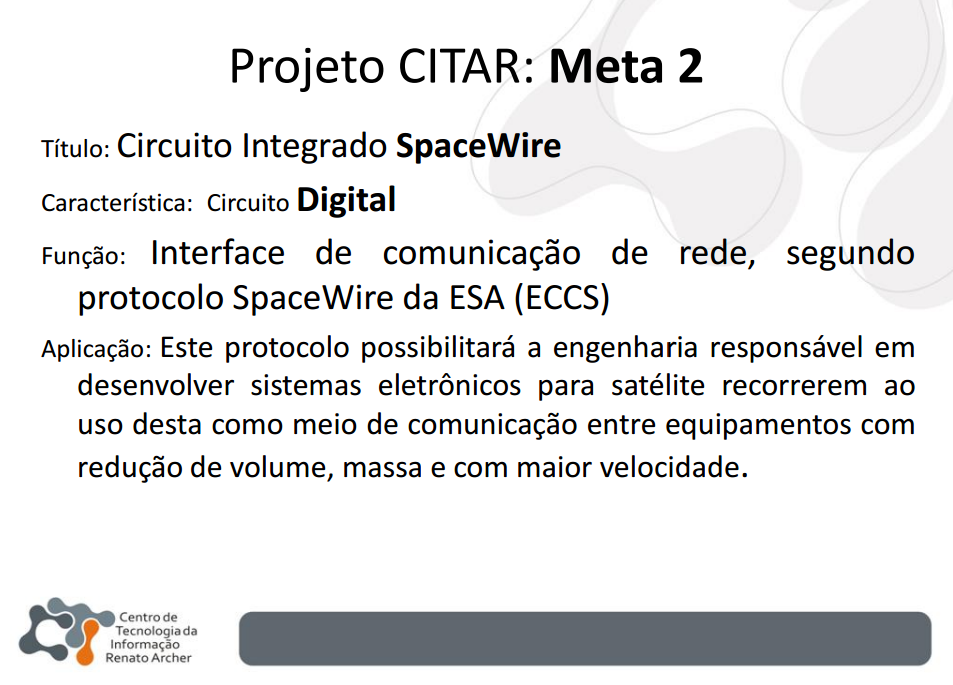
\includegraphics[scale = 0.55]{Imagens/ProjetoCitarMeta2}
	
	Fonte: site do IEAV Instituto de Estudos Avançados (2010, p. 9).\footnotemark[3]
	
	\label{Meta2}
\end{figure}

\let\thefootnote\relax\footnotetext[3]{Figura retirada da URL \url{http://www.ieav.cta.br/peice2010/Apresentacoes\_PEICE\%202010\_pdf/2010-11-29/0102-Saulo.pdf}. Acesso em: 7 out. 2015.}

\vfill

\begin{figure}[!htb]
	\centering
	\caption{Projeto CITAR - Meta 2.}
	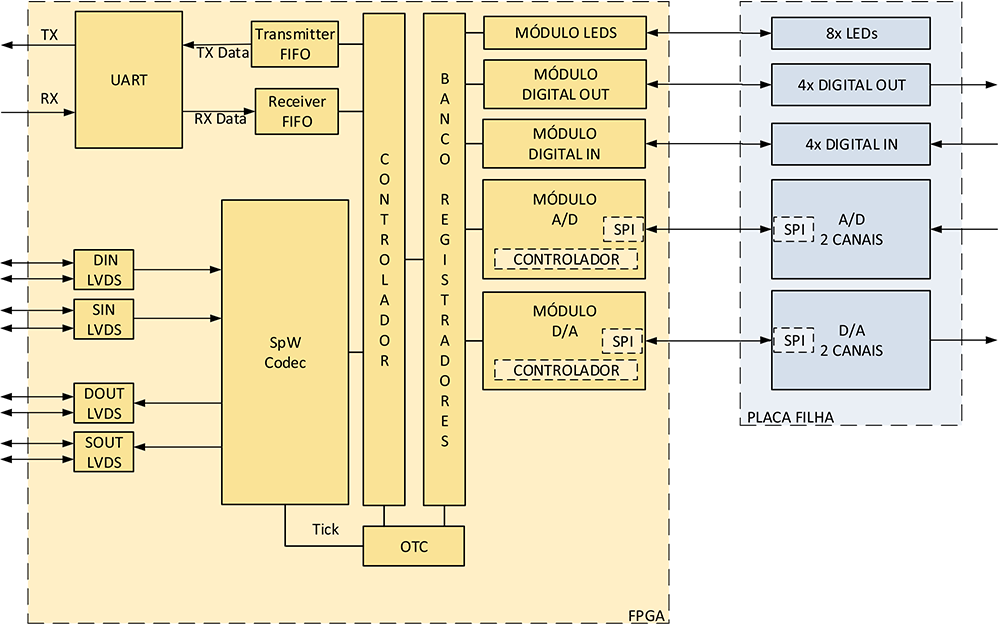
\includegraphics[scale = 1.7]{Imagens/Arch_ApSpW}
	
	Fonte: Elaborada pelo autor.
	
	\label{ArchSpW}
\end{figure}

}			% fim \afterpage
% ---

% ---
\section{Materiais e métodos}
Para o desenvolvimento do projeto foi utilizado:

\begin{itemize}
	\item Computador
	\item Software Xilinx ISE
	\item Placa de prototipagem GR-PCI-XC5V
	\item Cabo SpaceWire
\end{itemize}

Inicialmente foi realizado um estudo sobre as propriedades do protocolo SpaceWire. Em seguida, foram criados algumas aplicações utilizando o protocolo para melhor compreensão. Depois foi projetado a arquitetura proposta (Figura \ref{ArchSpW}) que possibilita o acesso aos conversores via protocolo SpW. Para todos os subsistemas um cenário de testes foi projetado, garantindo o perfeito funcionamento do sistema.

% ---


% ---
\section{Estudos, testes e simulações do codec SpaceWire}

\let\thefootnote\svthefootnote
O primeiro passo escolhido foi estudar sobre o protocolo de comunicação SpaceWire. Verificar seu funcionamento, os dados de entrada e de saída, a estrutura necessária para a sua aplicação, entre outros. O estudo se baseou inicialmente através da leitura do documento \textit{Space engineering: SpaceWire – Links, nodes, routers and networks}\footciteref{SpaceWire:Manual}, o qual descreve detalhadamente como devem ser construídos todos os níveis para sua implementação (nível das camadas física, de sinal, de caracteres, de pacotes de dados etc.). Procurou-se através deste estudo ter uma visão geral do protocolo, lembrando que o foco é a sua utilização e não a construção do mesmo.

O codec SpaceWire utilizado para estudo de teste e simulação foi desenvolvido por Jorge Luiz Nabarrete em seu trabalho de pós-doutorado no Instituto Mauá de Tecnologia em 2012.

Um dos primeiros testes com o codec foi verificar seu funcionamento ligando a saída do mesmo em sua entrada (loopback test). A simulação pôde ser visualizada através do software ISim (ISE Simulator) da Xilinx. Foram observadas várias características deste protocolo através desta simulação, entre elas, a taxa de envio de dados no início da transmissão e a alta prioridade no envio de TimeCode como está indicado na Figura \ref{SimulSpW_1}.

\begin{figure}[!htb]
	\centering
	\caption{Simulação codec SpW com interligação da saída com a entrada.}
	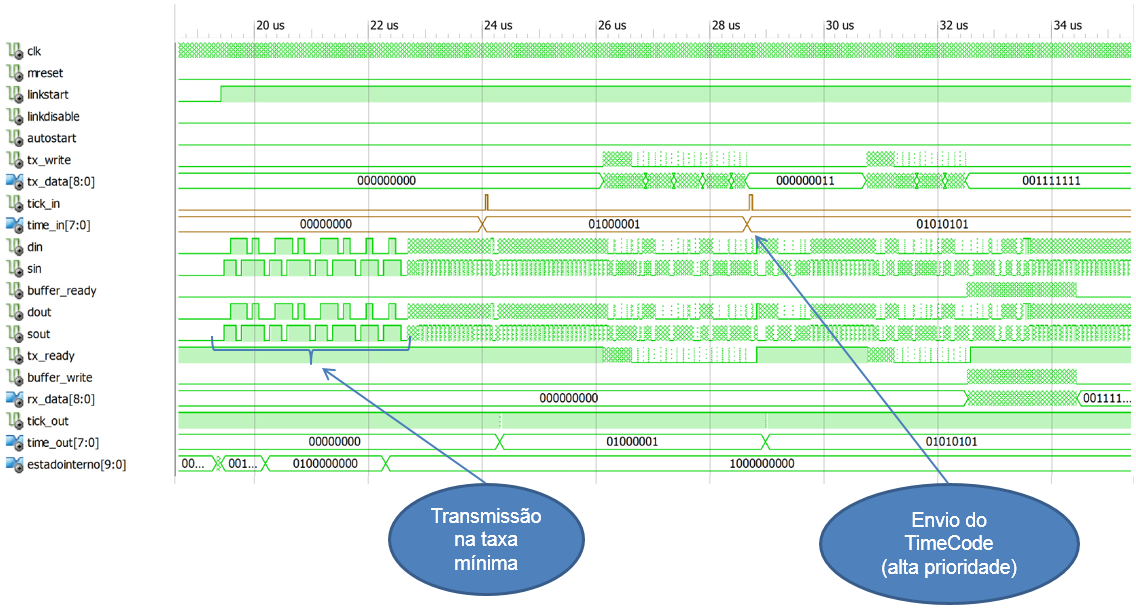
\includegraphics[scale = 0.7, angle = 90]{Imagens/SimulSpW_1}
	
	Fonte: Elaborada pelo autor.
	
	\label{SimulSpW_1}
\end{figure}

Outro teste realizado foi conectar o codec SpW que estava sendo analisado com o codec SpW que o coorientador Rafael Corsi Ferrão estava utilizando em seu projeto com a placa de desenvolvimento \textit{Altera DE4 Development and Education Board}\footnote{Altera DE4 Development and Education Board \url{http://www.terasic.com.tw/cgi-bin/page/archive.pl?Language=English\&CategoryNo=138\&No=\\501\&PartNo=1}}. Vale lembrar que os codecs SpW são de desenvolvedores diferentes. Após configurar a frequência de transmissão, vimos que os codecs se comunicavam corretamente.

Através da leitura, dos testes e simulações conseguiu-se criar uma boa base para o uso do protocolo SpaceWire e com isso dar prosseguimento no projeto.
% ---

% ---
\section{Arquitetura do sistema}

Após o estudo e análise do protocolo SpaceWire, iniciou-se o projeto da arquitetura do sistema. O objetivo desta etapa é estabelecer, de forma mais detalhada, os sinais de entrada e saída bem como os componentes a serem utilizados no sistema e suas interligações.

No inicio, a arquitetura proposta buscava mostrar de uma forma geral, o objetivo do projeto, como pode ser visualizada na figura \ref{Arch_1}.

Para a implementação do projeto, necessitou-se de uma arquitetura mais detalhada com os blocos necessários mais definidos. Após algumas modificações, chegou-se a arquitetura geral final que pode ser visualizada na figura \ref{Arch_ApSpW}. Pode-se observar a estrutura dos blocos que estão contidos na FPGA e os blocos na Placa Filha\footnote{Placa Filha: Nome dado a placa construída no projeto, a qual contém leds, saídas e entradas digitais e os conversores A/D e D/A.}.

Também foi feito uma pequena arquitetura (figura \ref{Arch_conversores}) mostrando com maior detalhe a comunicação entre os módulos A/D e D/A com seus respectivos conversores. Essa pequena arquitetura ajudou na implementação do código VHDL dos módulos, pois permitiu visualizar as entradas e saídas necessárias da comunicação SPI (Serial Peripheral Interface) com os conversores.

Os conversores utilizados no projeto são: o analógico-digital MCP3204\footnote{\label{MCP3204}Datasheet do conversor A/D MCP3204: \url{http://ww1.microchip.com/downloads/en/DeviceDoc/21298c.pdf}. Acesso em: 12 out. 2015.} e o digital-analógico MCP4922\footnote{\label{MCP4922}Datasheet do conversor D/A MCP4922: \url{http://ww1.microchip.com/downloads/en/DeviceDoc/22250A.pdf}. Acesso em: 12 out. 2015.}, ambos da Microchip. Foram escolhidos estes conversores pois oferecem interface de comunicação SPI, possuem no mínimo dois canais de leitura/escrita e uma boa resolução (12 bits). Procurou-se com estes conversores criar uma aplicação que pudesse ser bem genérica, podendo conectá-los a quatro equipamentos como motores e sensores.

\begin{figure}[!htb]
	\centering
	\caption{Primeira arquitetura do projeto Aplicação SpaceWire.}
	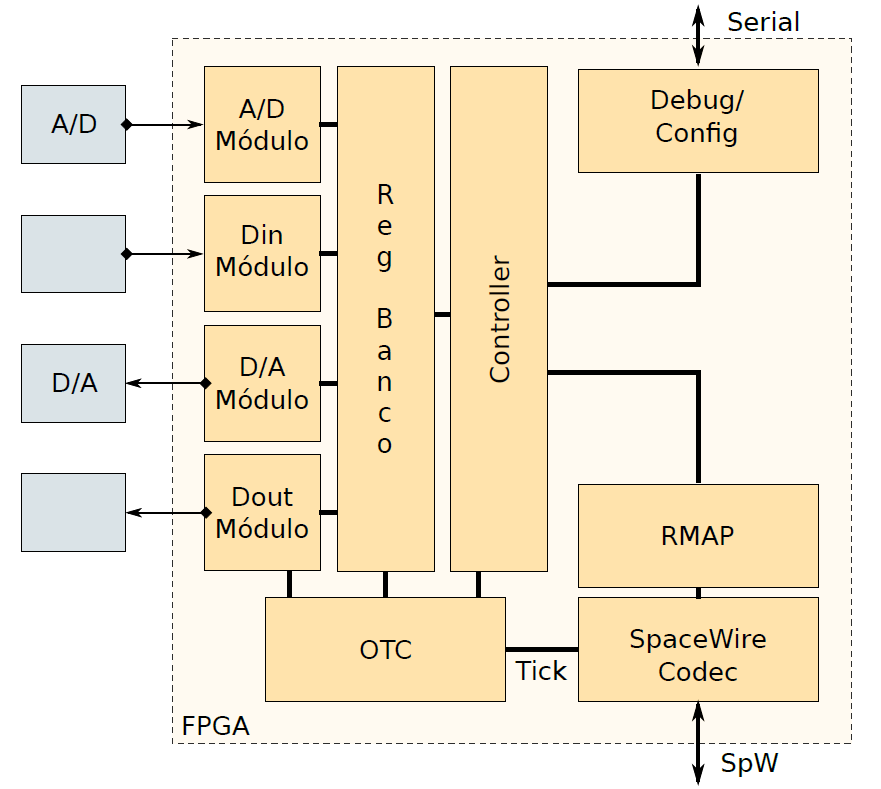
\includegraphics[scale = 0.5]{Imagens/Arch_1.png}
	
	Fonte: Elaborada pelo autor.
	
	\label{Arch_1}
\end{figure}

\begin{figure}[!htb]
	\centering
	\caption{Arquitetura geral do projeto Aplicação SpaceWire.}
	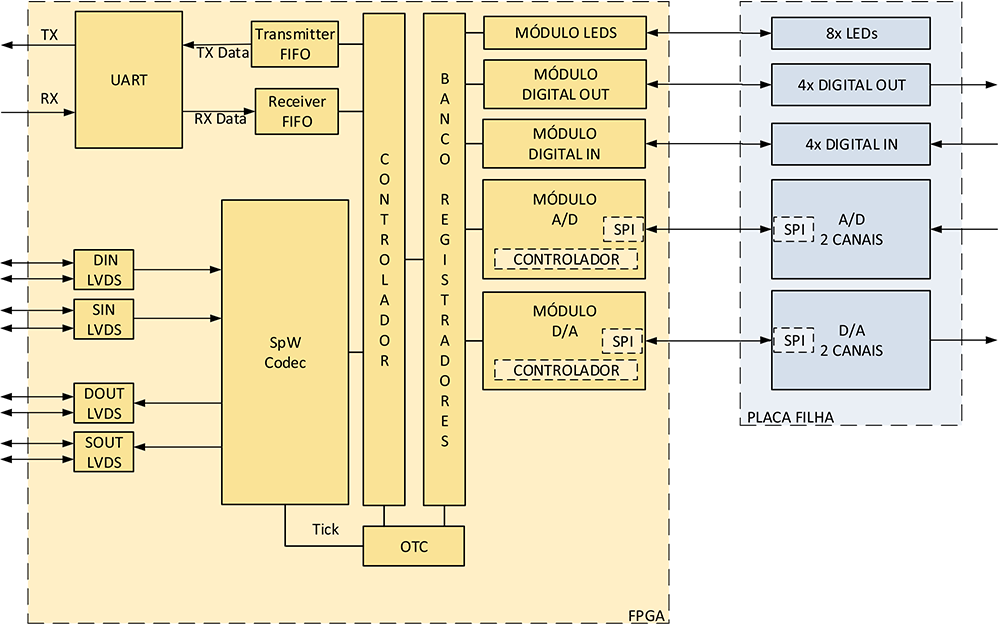
\includegraphics[scale = 1.85]{Imagens/Arch_ApSpW}
	
	Fonte: Elaborada pelo autor.
	
	\label{Arch_ApSpW}
\end{figure}

\begin{figure}[!htb]
	\centering
	\caption{Arquitetura entre os módulos A/D e D/A e seus respectivos conversores.}
	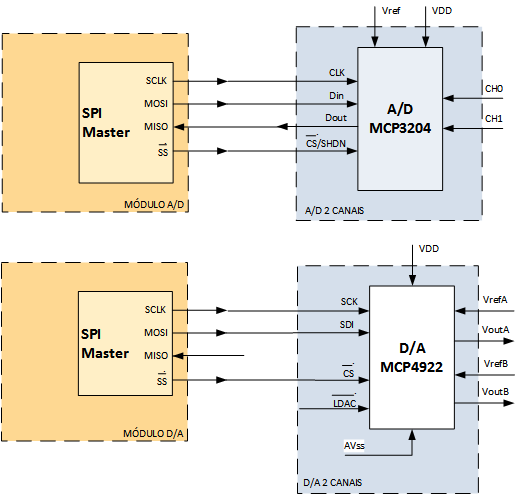
\includegraphics[scale = 0.9]{Imagens/Arch_conversores}
	
	Fonte: Elaborada pelo autor.
	
	\label{Arch_conversores}
\end{figure}

% ---

\vfill

% ---
\section{Construção do hardware (Placa Filha)}

Foi construído um hardware, chamado Placa Filha (figura \ref{PlacaFilha}), contendo: oito leds, seis entradas/saídas digitais, um coversor A/D MCP3204 e um convesor D/A MCP4922. Esta placa foi projetada com o intuito de ser acoplada a placa de desenvolvimento GR-PCI-XC5V\footciteref{Gaisler:Online} através de uma placa expansora de pinos GR-CPCI-TEST da Aeroflex Gaisler (figura \ref{cpci-test} e figura \ref{PlacaFilha_GRPCI}).

A placa foi projetada utilizando o programa EAGLE PCB Design Software\footciteref{Eagle:online} e confeccionada em uma máquina LPKF disponibilizada pelo Instituto Mauá de Tecnologia. O diagrama esquemático da placa está em anexo no Apêndice A no final do relatório.

Esta placa permite que testes práticos possam ser realizados e mostrar o real funcionamento do sistema.

\begin{figure}[!htb]
	\centering
	\caption{Foto da Placa Filha conectada na placa expansora GR-CPCI-TEST.}
	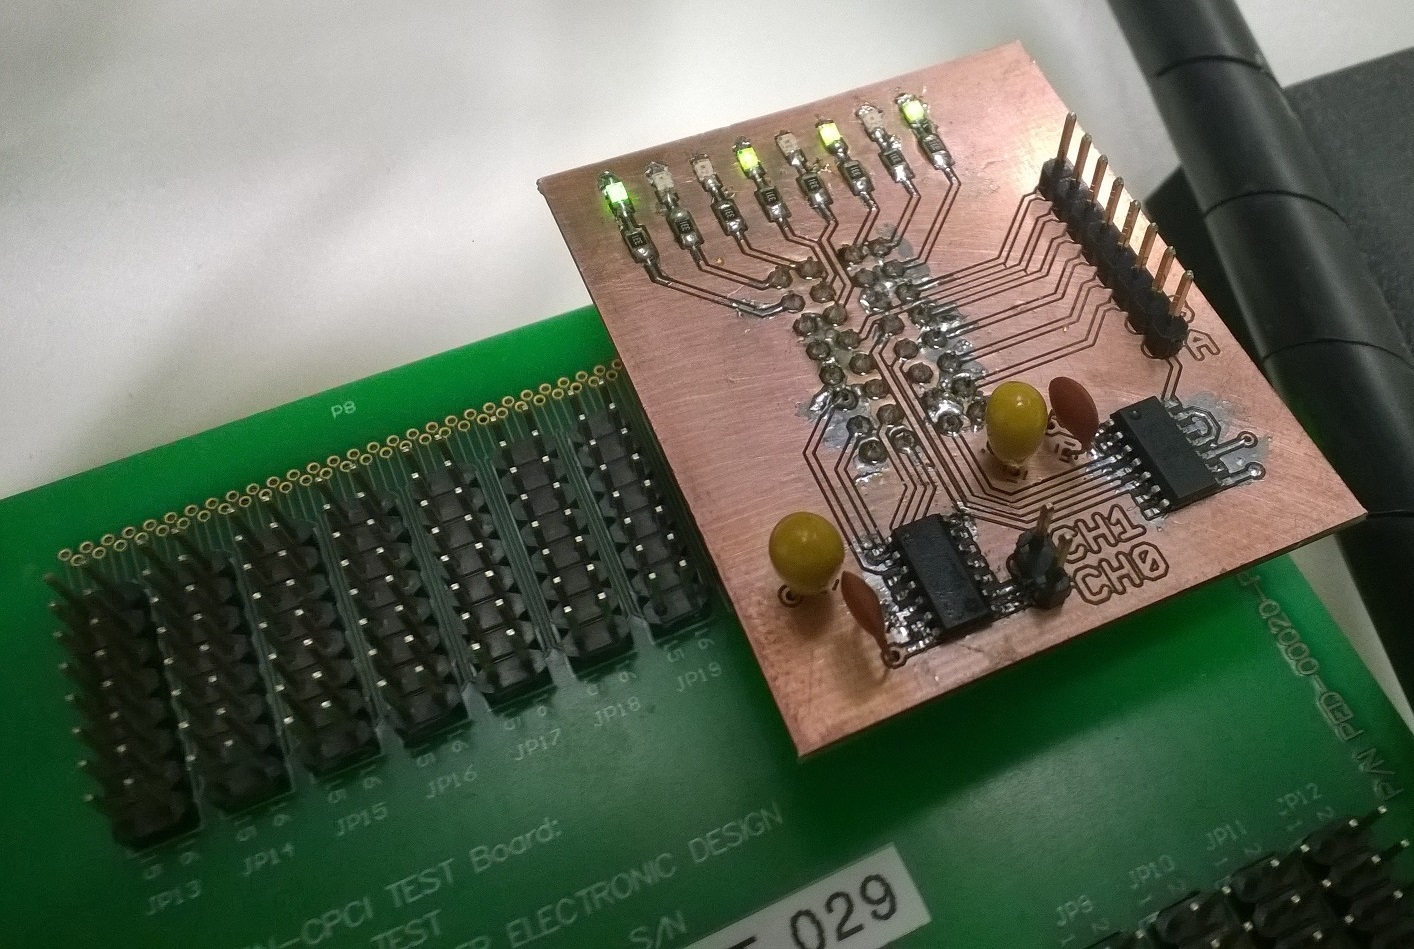
\includegraphics[scale = .4]{Imagens/PlacaFilha}
	
	Fonte: Elaborada pelo autor.
	
	\label{PlacaFilha}
\end{figure}

\begin{figure}[!htb]
	\centering
	\caption{GR-CPCI-TEST}
	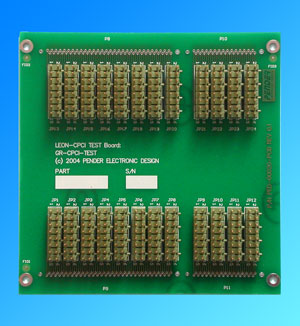
\includegraphics[scale = .9]{Imagens/cpci-test}
	
	Fonte: GAISLER.
	
	\label{cpci-test}
\end{figure}

\begin{figure}[H]
	\centering
	\caption{Placa Filha, GR-PCI-TEST e GR-PCI-XC5V.}
	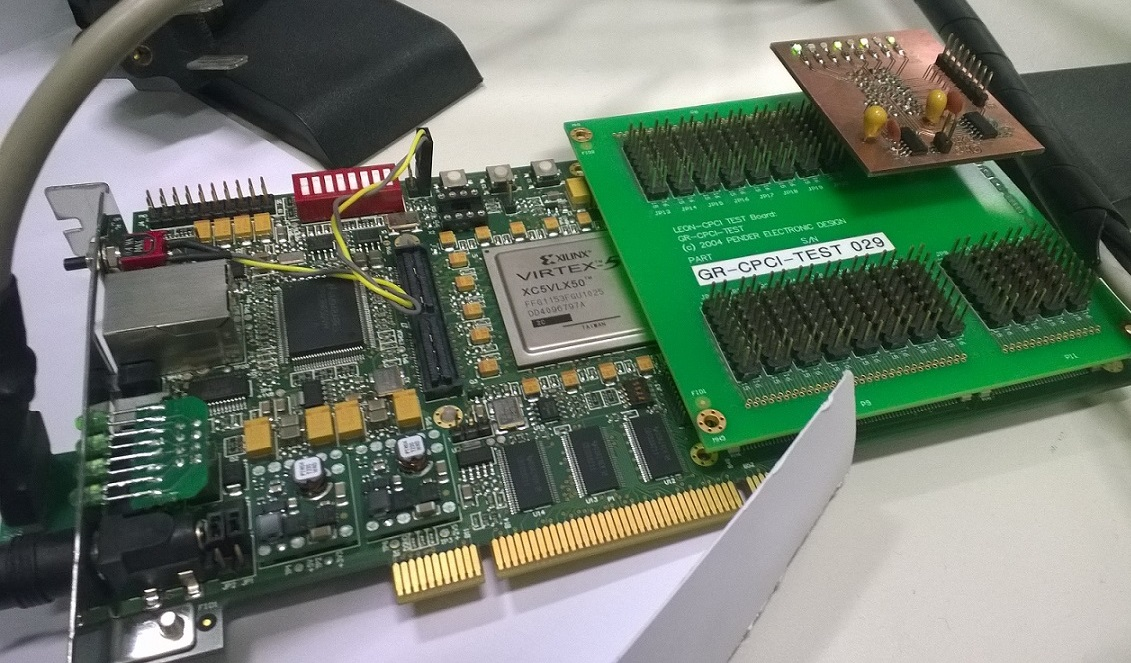
\includegraphics[scale = .8, angle = 90]{Imagens/PlacaFilha_GRPCI}
	
	Fonte: Elaborada pelo autor.
	
	\label{PlacaFilha_GRPCI}
\end{figure}

% ---

\section{Implementação, simulação e teste do módulo digital-analógico com o conversor D/A MCP4922}

Através da Placa Filha pôde-se finalmente realizar testes com os conversores. Mas antes disso, é necessário fazer a implementação dos módulos e realizar simulações em software antes de efetivamente executá-los na prática. É muito importante o uso da simulação em software, pois se o subsistema não funcionar na simulação, muito provavelmente não funcionará na prática.

Para a implementação do módulo digital-analógico através da programação em VHDL, construiu-se, primeiramente, um diagrama de blocos do controlador do módulo para melhor compreensão e organização da estrutura do código. Este diagrama é mostrado na figura \ref{controlador_DAC}. Foi utilizado como referência para a construção do diagrama a máquina de Moore onde as saídas são determinadas pelo estado corrente apenas (e não pela entrada). 

O controlador do módulo D/A controla os sinais do módulo SPI que é por onde os dados são enviados e recebidos do conversor. Inicialmente o controlador espera chegar um dado novo no registrador para começar o processo de envio ao canal especificado do conversor. Após iniciado o processo de envio do dado, o mesmo entra em um novo estado de espera até que o último bit seja enviado. Logo depois, o controlador verifica se há um dado a ser enviado ao outro canal do conversor, evitando assim com que um canal tenha maior prioridade do que o outro.

Após a implementação em código VHDL, realizou-se a simulação deste sistema através do software ISim (ISE Simulator) da Xilinx, mostrado na figura \ref{ISim_DAC}. Pode-se observar que quando o dado a ser enviado chega por completo ao registrador nos endereços 30, 31 e 32, o controlador manda este dado para o SPI, que por sua vez envia o dado ao conversor MCP4922 através do sinal spi\_mosi\_o. O pacote de dados completo é composto por quatro bits de configuração do conversor (quatro bits menos significativos do endereço 30), quatro bits mais significativos de dados (quatro bits menos significativos do endereço 32) e mais oito bits de dados restantes (endereço 31). O comando de escrita necessário para o conversor MCP4922 é mostrado na figura \ref{WriteCommandMCP4922}.

Por fim, foi realizado um teste na prática para ver este sistema funcionando. Neste teste estava sendo utilizado: o banco de registradores, o módulo A/D e o conversor A/D MCP4922. O registrador ficava recebendo dados em um endereço específico e enquanto isso o controlador do módulo verificava se havia um dado novo a ser enviado ao D/A. Toda vez que um dado era escrito no registrador, o controlador enviava este dado via SPI para o conversor MCP4922. O sinal analógico do conversor pôde ser observado através de um osciloscópio. A foto do teste realizado na prática pode ser visualizada na figura \ref{teste_conversor_DAC}.

\begin{figure}[!htb]
	\centering
	\caption{Diagrama de blocos do controlador do módulo digital-analógico.}
	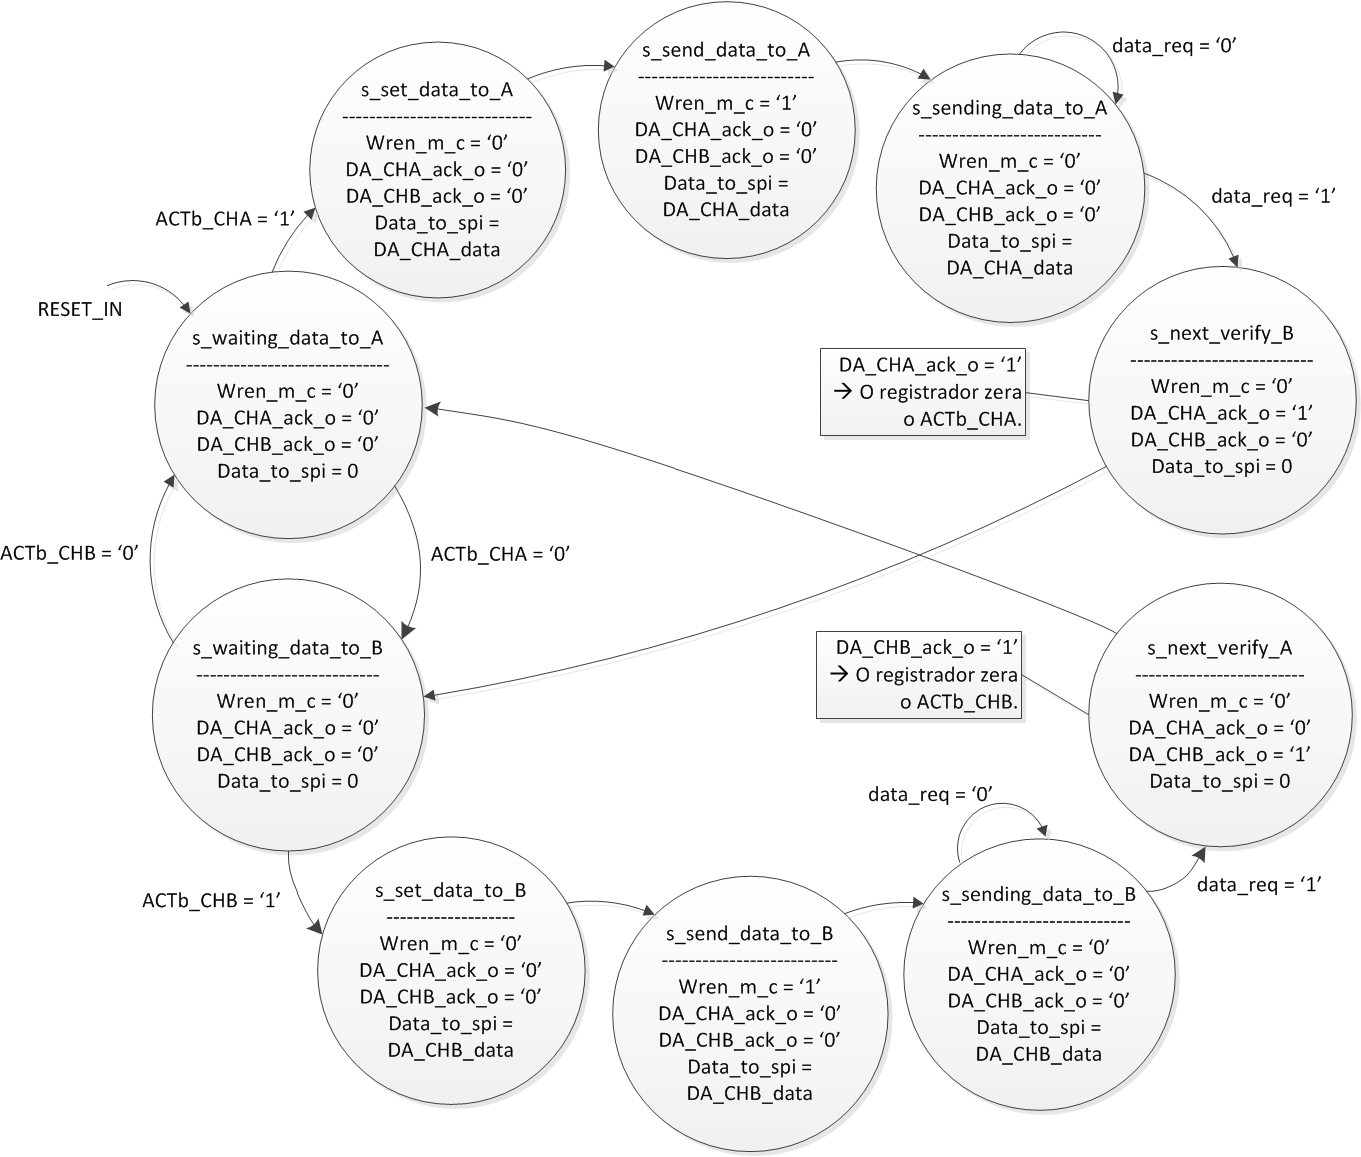
\includegraphics[scale = .9]{Imagens/controlador_DAC}
	
	Fonte: Elaborada pelo autor.
	
	\label{controlador_DAC}
\end{figure}

\begin{figure}[!htb]
	\centering
	\caption{Simulação do módulo digital-analógico utilizando o software ISim.}
	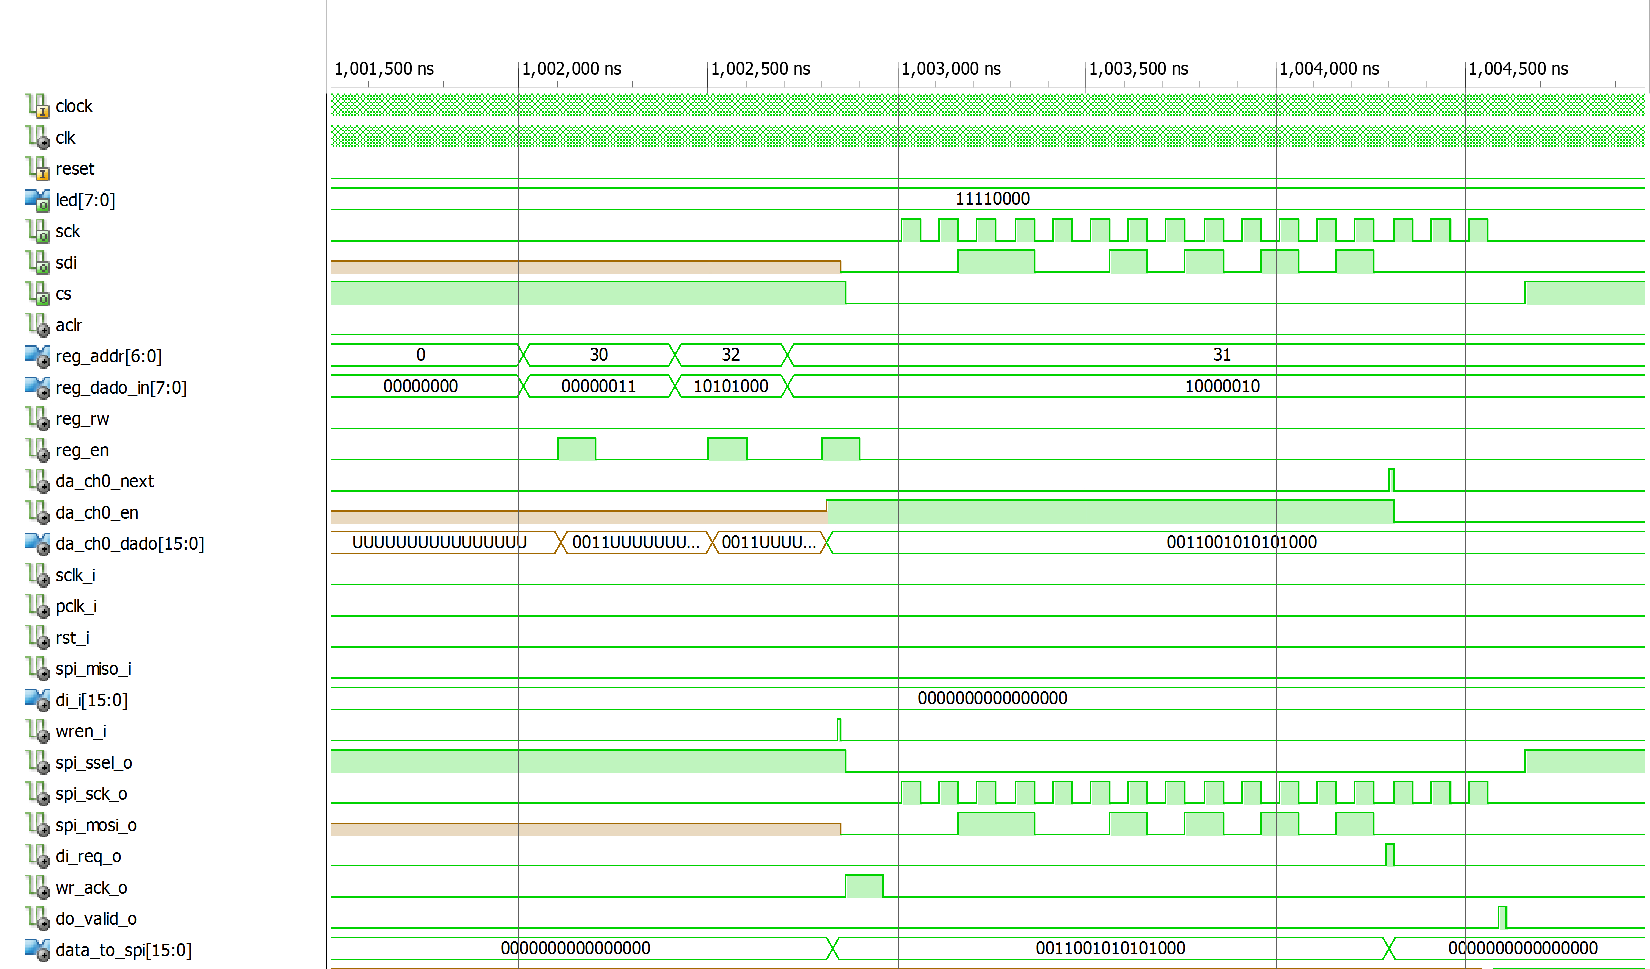
\includegraphics[scale = .8, angle = 90]{Imagens/ISim_DAC_.pdf}
	
	Fonte: Elaborada pelo autor.
	
	\label{ISim_DAC}
\end{figure}

\begin{figure}[!htb]
	\centering
	\caption{Comando de escrita para o conversor MCP4922.}
	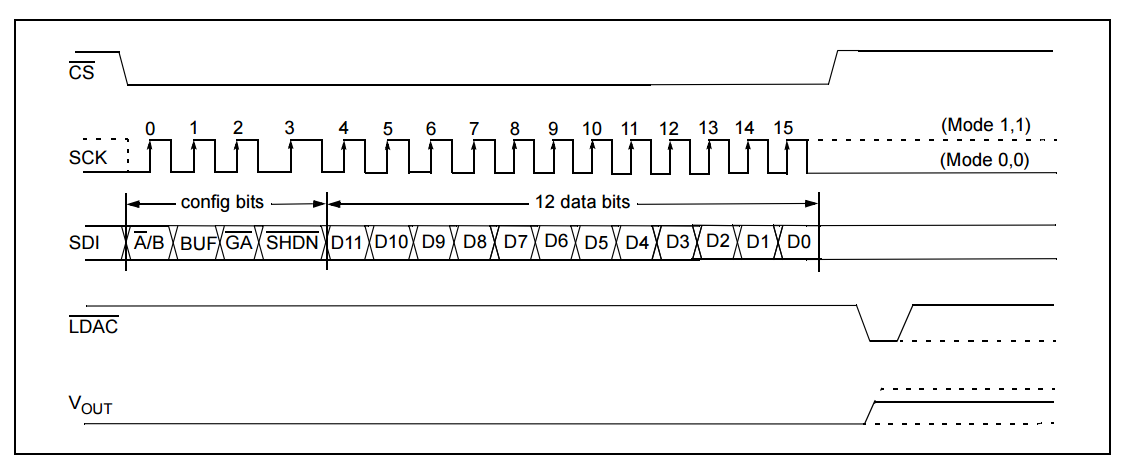
\includegraphics[scale = .5]{Imagens/WriteCommandMCP4922}
	
	Fonte: Elaborada pelo autor.
	
	\label{WriteCommandMCP4922}
\end{figure}

\begin{figure}[!htb]
	\centering
	\caption{Teste prático do controlador D/A MCP4922 utilizando osciloscópio.}
	\includegraphics[scale = .7, angle = 90]{Imagens/teste_conversor_DAC}
	
	Fonte: Elaborada pelo autor.
	
	\label{teste_conversor_DAC}
\end{figure}

% ---

% ----------------------------------------------------------
% PARTE
% ----------------------------------------------------------
\part{Considerações finais}
% ----------------------------------------------------------

% ---
% Capitulo : Atividades a realizar
% ---
\chapter{Atividades a realizar}

Falta realizar o teste prático do módulo A/D (utilizando controlador, registrador e o módulo SPI), configurações do módulo da comunicação serial e interligar todos os módulos e subsistemas. Para o projeto também é necessário definir o protocolo de comunicação para que o usuário externo, via SpaceWire ou comunicação serial, possa acessar e controlar os componentes da placa. A escolha do tamanho do registrador com endereços específicos para cada elemento do sistema está praticamente finalizado.
% ---

% ----------------------------------------------------------
% Finaliza a parte no bookmark do PDF
% para que se inicie o bookmark na raiz
% e adiciona espaço de parte no Sumário
% ----------------------------------------------------------
\phantompart

% ---
% Conclusão
% ---
\chapter{Conclusão}

Com uma forma abrangente na área da  engenharia eletrônica, o estágio proporcionou a realização de várias atividades práticas através do desenvolvimento de hardware, software e firmware.

Além de poder colocar em prática os conhecimentos adquiridos durante a graduação no Curso de Engenharia Eletrônica, pude com o estágio aprender a utilizar novas técnicas e ferramentas relacionadas a projetos e desenvolvimento de sistemas eletrônicos. Foram realizados constantes estudos e análises através da leitura de datasheets para implementação dos componentes e protocolos, foi possível implementar hardware em FPGA através de programação em código VHDL, realizar simulações em softwares e construir um hardware versátil que pudesse ser acoplado a placa de desenvolvimento utilizada.

De uma forma geral, além da parte técnica necessária para o desenvolvimento das tarefas, o trabalho também permitiu a socialização com alunos e pesquisadores que utilizam o laboratório NSEE para desenvolver seus projetos através da troca de informações, conhecimentos e experiências no dia a dia e nas reuniões estipuladas entre equipes de diferentes áreas.

% ---



% ----------------------------------------------------------
% ELEMENTOS PÓS-TEXTUAIS
% ----------------------------------------------------------
\postextual
% ----------------------------------------------------------

% ----------------------------------------------------------
% Referências bibliográficas
% ----------------------------------------------------------
\bibliography{Bibliografia}


% ----------------------------------------------------------
% Glossário
% ----------------------------------------------------------
%
% Consulte o manual da classe abntex2 para orientações sobre o glossário.
%
%\glossary

% ----------------------------------------------------------
% Apêndices
% ----------------------------------------------------------

% ---
% Inicia os apêndices
% ---
\begin{apendicesenv}

% Imprime uma página indicando o início dos apêndices
\partapendices

% ----------------------------------------------------------
\chapter{Diagrama esquemático da Placa Filha}
% ----------------------------------------------------------

Na próxima página é anexado o diagrama esquemático da Placa Filha. Para projetá-lo foi utilizado o programa EAGLE PCB Design Software.

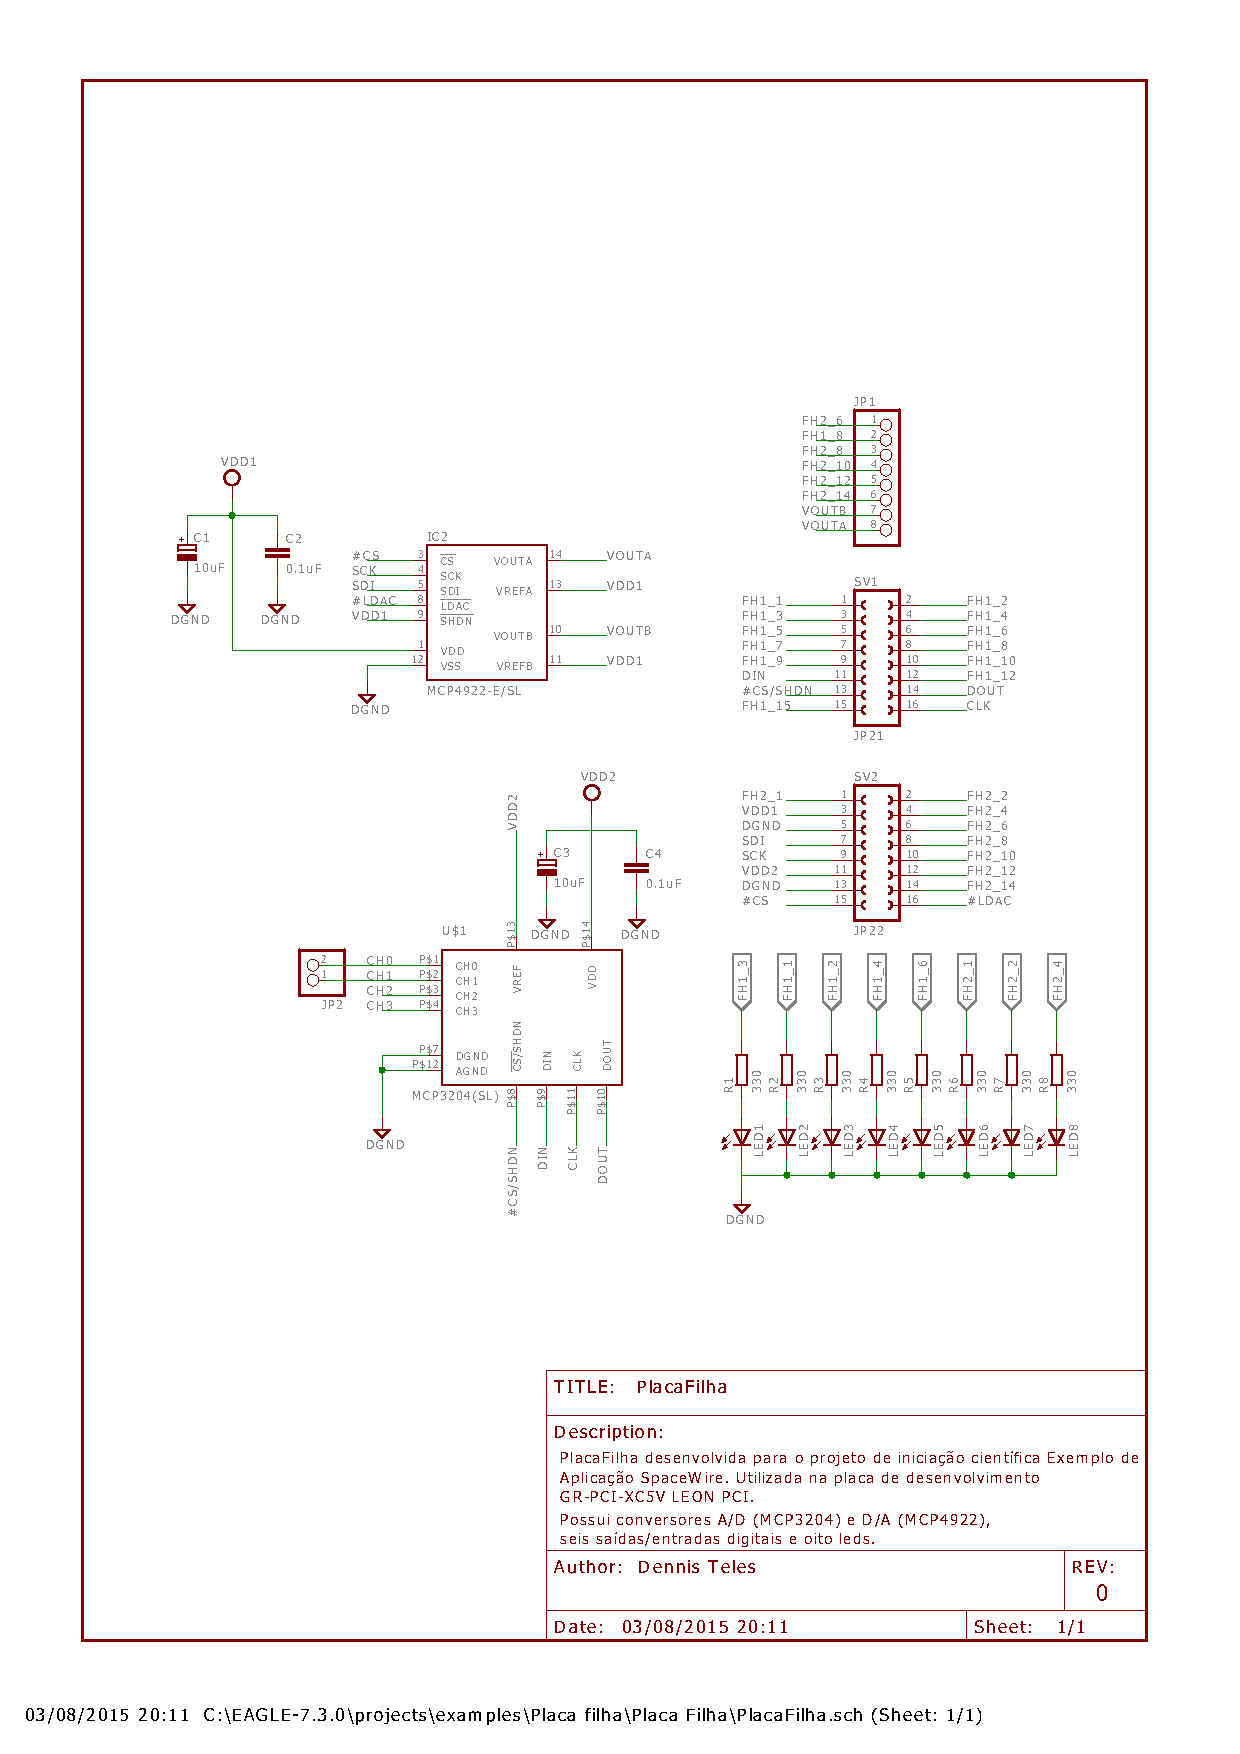
\includepdf[pages={1}]{Imagens/PlacaFilha_schematic.pdf}

\end{apendicesenv}
% ---

\iffalse

% ----------------------------------------------------------
% Anexos
% ----------------------------------------------------------

% ---
% Inicia os anexos
% ---
\begin{anexosenv}

% Imprime uma página indicando o início dos anexos
\partanexos

% ---
\chapter{Morbi ultrices rutrum lorem.}
% ---
\lipsum[30]

% ---
\chapter{Cras non urna sed feugiat cum sociis natoque penatibus et magnis dis
parturient montes nascetur ridiculus mus}
% ---

\lipsum[31]

% ---
\chapter{Fusce facilisis lacinia dui}
% ---

\lipsum[32]

\end{anexosenv}

\fi

%---------------------------------------------------------------------
% INDICE REMISSIVO
%---------------------------------------------------------------------
\phantompart
\printindex
%---------------------------------------------------------------------

\chapter*{\newpage}

\vspace*{5cm}
\setlength{\parskip}{7em}
\assinatura{\textbf{Dennis Teles dos Santos}\\ RA: 09.03046-8\\ IMT-Instituto Mauá de Tecnologia}
	
\assinatura{\textbf{Vanderlei Cunha Parro}\\ Orientador}

\definecolor{light-gray}{gray}{0.9}	
	
\assinatura{\textcolor{light-gray}{\textbf{\underline{\hspace{6cm}}}}\\ Examinador}	




\end{document}
